 \documentclass{sig-alternate}
\usepackage{graphicx}
\usepackage{subfigure}
\usepackage{stmaryrd}

% PASSW for PEPM: pe06stups
% Mauricio: m.varea@ecs.soton.ac.uk,michael68


\newcommand{\logen}[2]{$\underbrace{\texttt{#2}}_{{\footnotesize #1}}$}
\newcommand{\unfold}[1]{\logen{unfold}{#1}}
\newcommand{\memo}[1]{\logen{memo}{#1}}

% Standard Definitions

\newcommand{\NN}{\mbox{${I\!\!N}$}}
\newcommand{\RR}{\mbox{${I\!\!R}$}}
\newcommand{\ZZ}{\mbox{${Z\!\!\!Z}$}}

\def\mymath#1{\relax\ifmmode#1\else$#1$\fi}
\newcommand{\sembra}[2]{\mymath{[\![#1]\!]_{\rm#2}}}
\newcommand{\sem}[1]{\mymath{[\![#1]\!]}}

\newcommand{\theoremstart}[2]{{\bf #1 #2}}
\newcommand{\theoend}{\hspace*{\fill}\(\Box\)}

\newcounter{defcounter}[section]
\renewcommand{\thedefcounter}{\thesection.\arabic{defcounter}}

\newenvironment{algorithm}%
{\refstepcounter{defcounter} \begin{trivlist} \item[]%
\theoremstart{Algorithm}{\thedefcounter}}%
{\end{trivlist}}

\newenvironment{zitemize}% zero - line spacing itemize environment
   {\begin{list}{--}{
   \setlength{\itemsep}{0 pt}
   \setlength{\parsep}{0 pt}
   \setlength{\topsep} {0 pt} }}% the end stuff
   {\end{list}}
\newenvironment{pitemize}% zero - line spacing itemize environment for programs
   {\begin{list}{}{
   \setlength{\itemsep}{0 pt}
   \setlength{\parsep}{0 pt}
   \setlength{\topsep} {2 pt} }}% the end stuff
   {\end{list}}
\newcommand{\mikearraystretch}{1}
\newcommand{\var}[1]{#1}
\newcommand{\svar}[1]{\mbox{{\scriptsize #1}}}

\newcommand{\larr}{\leftarrow}


\newcommand{\diff}{\mathit{\backslash\!==}}
\newcommand{\dif}{\mathit{\backslash\!=}}

\newcommand{\MSG}[2]{\mathit{msg}(#1,#2)}
\newcommand{\MGU}[1]{\mathit{mgu}(#1)}


\newcommand{\homeo}{\unlhd}
\newcommand{\nothomeo}{\not\!\unlhd}
\newcommand{\homeostrict}{\lhd}


\newcommand{\ignore}[1]{} % {{\tt \small ignore(#1)}}
\newcommand{\forExperts}[1]{} % {{\small {\bf For Experts Only:}\\ #1}}
\newcommand{\comment}[1]{}

\numberofauthors{2}
\title{The Ecce Online Specialiser and its Web Interface}
\author{
\alignauthor Michael Leuschel$^*$\\
       \affaddr{University of D\"{u}sseldorf, Germany}\\
       \email{leuschel@cs.uni-duesseldorf.de}
\alignauthor Mauricio Varea\thanks{The authors have been partially supported by the Information Society Technologies programme of the European Commission, Future and Emerging Technologies under the IST-2001-38059 ASAP project.}\\
       \affaddr{University of Southampton, United Kingdom}\\
       \email{m.varea@ecs.soton.ac.uk}
}
\date{}
\CopyrightYear{2005}

\pagestyle{plain} %empty,plain

\begin{document}


\maketitle

\begin{abstract}
We present the {\sc ecce} system, a fully automatic {\em online} specialiser for logic
programs implemented in Prolog.
We also discuss a new modular implementation of {\sc ecce}, carried out in Ciao Prolog, 
which allows people to perform specialisation of logic programs, either via its command-line interface or a web interface implemented in PHP.
%{\sc ecce}'s graphical user interface can be used either remotely or locally.
\end{abstract}


% ----------------------------------------------
\section{The Ecce System}

{\em Program specialisation}, also called
 {\em partial evaluation\index{partial evaluation}\/} or
 {\em partial deduction\index{partial deduction}},
  is an automatic technique for program optimisation.
The central purpose is to specialise a given source program
 for a particular application domain.
%This is (mostly) done by a {\em well-automated\/} application of parts
% of the Burstall and Darlington unfold/fold\index{unfold/fold}
%  transformation framework.
Program specialisation encompasses traditional
 compiler
 optimisation techniques,
% such as {\em constant folding\index{constant folding}\/} and {\em
% in-lining\index{in-lining}},
 but uses more aggressive
 transformations, yielding both much
 greater speedups and more difficulty in
 controlling the transformation process.

{\sc ecce} is a specialiser for logic programs.
{\sc ecce} is an online system, i.e., it requires no preliminary
 annotation phase and takes all its decisions automatically during
 specialisation.
  Its  input are
 pure Prolog programs (with built-ins, as long as they are used in a declarative
  manner).
The control of  {\sc ecce} is
  separated  into two components \cite{MartensGallagher:ICLP95}:

\begin{itemize}
\item The {\em global control\/} (also called control of polyvariance)
  decides {\em which\/} specialised predicates are present in
   the residual program and ensures that all calls that occur at runtime
   are an instance of some specialised atom.
\item The {\em local control\/} (also called unfolding) is responsible for the
 construction of  the residual clauses for each specialised atom.
\end{itemize}


Some of the particularities of the {\sc ecce} system are:
\begin{zitemize}
\item For the local control {\sc ecce} uses determinacy (with lookahead) to decide
 which atoms should be unfolded
 and homeomorphic embedding  (see, e.g., \cite{Leuschel:NeilFest02}) to ensure
 termination (i.e., decide which ones should not be unfolded).
 \item For the global control {\sc ecce} uses both characteristic trees and homeomorphic embedding
  \cite{LeuschelMartens:Dagstuhl96,LeuschelMartensDeSchreye:Toplas}.
  The characteristic trees \cite{Gallagher91:ngc}
   are used to capture the specialisation performed
   on a call, and are used to control the polyvariance: if two calls have a different
    characteristic tree then they are specialised in a different way and combining
    them would result in a loss of specialisation.
   The homeomorphic embedding relation
   is used to ensure that only finitely many atoms are specialised.
   For generalisation, the most specific generalisation ({\em msg}) \cite{LassezMaherMarriott:fddlp88} is used.
 \item {\sc ecce} caters for
  {\em conjunctive partial deduction\/} \cite{LeuschelDeSchreyeDeWaal:JICSLP96,CPD:megapaper}.
  Essentially, this makes it possible to specialise a conjunction of atoms together
   rather than in isolation, opening up the door for optimisations such as
    deforestation (getting rid of intermediate datastructures) and tupling
    (merging multiple visits of some datastructure).
 \item Redundant argument filtering \cite{LeuschelSorensen:RAF} is another
  ingredient of {\sc ecce} which filters out various useless arguments in the
   specialised programs.
\end{zitemize}

Various abstract interpretation techniques have been integrated
 into {\sc ecce}
(more specific version \cite{MarriottNaishLassez:AMAI90} calculation in
\cite{LeuschelDeSchreye:PLILP96}, and regular types in
\cite{LeuschelGruner:LOPSTR2001}).
It is also possible to develop custom local and global control predicates, as well as override
 various other components of {\sc ecce}.
Note that {\sc ecce} does not support non-declarative Prolog programs (i.e., Prolog
 programs which rely on the left-to-right selection rule):
  while this restricts the applicability of {\sc ecce},%
\footnote{For non-declarative programs  {\sc mixtus} \cite{Sahlin93:ngc} or
 {\sc logen}  \cite{LeuschelEtAl:TPLP03} are better alternatives.}
 it also enables {\sc ecce} to perform
  more powerful optimisations (e.g., replacing infinite by finite failure).
 However, {\sc ecce} is still guaranteed (in default settings) to preserve the order of solutions.

%\cite{Leuschel:JICSLP98},

\section{Applications}

Evaluations of {\sc ecce}'s performance on a variety of benchmarks
 can be found in \cite{LeuschelMartensDeSchreye:Toplas}
 and in \cite{JorgensenLeuschelMartens:CPPD,CPD:megapaper} for
 the conjunctive partial deduction component.
Results are compared, amongst others, against
 {\sc mixtus} \cite{Sahlin93:ngc}, {\sc sp}  \cite{Gallagher91:ngc} and {\sc paddy} \cite{Prestwich:PEPM93}.

There have been many applications of {\sc ecce} outside of the classical
 objective of speeding up logic programs.
{\sc ecce} has been applied to program
 inversion \cite{GlueckLeuschel:Inversion},
 inductive theorem proving \cite{Leuschel:Lopstr03}
  and to solve
planning problems of the fluent calculus \cite{LehmannLeuschel:LPAR2000}.

{\sc ecce} has been used for
 infinite state model checking in \cite{LeuschelMassart:LOPSTR99} in general
  and for the coverability problem of Petri nets \cite{LeuschelLehmann:Coverability,LeuschelLehmann:CL2000} in particular.
It has been shown that a special case of the control algorithm of {\sc ecce} corresponds to the Karp-Miller procedure
for Petri nets.
 Recently, {\sc ecce} has also been applied for verification of
  Object Petri nets in \cite{FarwerLeuschel:PPDP04}.

In \cite{LeuschelVidal:ESOP05}
 it was shown that by changing {\sc ecce}'s post-processor it was possible
  to obtain a precise slicing algorithm for logic programs.
Finally, {\sc ecce} has been used as a pre-processor for 
 termination analysers 
  \cite{TamaryCodish:WST04}, with the aim of proving more programs terminating.
%Serbrenik, Adornments ??

\section{A modular implementation in\\ Ciao Prolog}

{\sc ecce} was originally implemented in BIM Prolog and later ported to SICStus. The majority of {\sc ecce}'s evolution has taken place while being written in SICStus Prolog. 
However, this implementation suffered from a significant increment in complexity, and very little could be done to alleviate this as the tool was not written in a modular way. On the advent of the ASAP project we decided twofold: (a) to port the tool another time, to Ciao Prolog,
 while maintaining compatibility with SICStus Prolog, and (b) to use modularity, in order to obtain a cleaner implementation of {\sc ecce}.
As a further advantage, 
 Ciao's compiler, {\tt ciaoc}, allows to easily create stand-alone executables and command-line tools.
The {\sc ecce} executable operates in three different modes:

\begin{zitemize}
\item in interactive mode,
\item in scripted mode for benchmarking, and
\item via a command-line interface (CLI).
\end{zitemize}

In the {\em interactive} mode, users to interact with the tool via the text-mode menu shown in Figure~\ref{fig:interactive}. The mode {\em for benchmarking} was created to allow the more intrepid user to automate their interaction with {\sc ecce}. In this way, the user could simple pass a list of tasks to the tool, instead of selecting a set of options from the interactive menu. This is very useful for benchmarking. Finally, an extensive CLI was added to {\sc ecce} in order to efficiently operate the tool from different front-ends. Figure~\ref{fig:CLI} shows the different switches that can be used in this mode.  

\begin{figure}[!ht]
\centering
\begin{minipage}[t]{.9\textwidth}
\begin{scriptsize}\begin{verbatim}
[MV-Computer:~/] mv% ./ecce -i
=> h
 ECCE 2.0
 The Partial Evaluator based on Characteristic Atoms 
 and Global Trees

  database name: compat
clauses stored in database: 0
database contains *no* facts

 Command Summary:
  c: Clear clause database
  e: set dEbugging on/off
  f: choose File for output
  h: Help (also ?)
  i: Insert specialised program into clause database
  l: List clause database
  o: turn type checking Off
  p: Partially evaluate an atom or goal
  r: Read clauses into database
  s: Set Parameters
  v: set user expert leVel on/off
  w: Write specialised program to file
  W: Write specialised program as Isabelle theory file
  x: eXit (also a and q)
  ----------------------------------- 
  d: Determinate (post-)unfolding
  m: Msv analysis
  n: eNable abstract partial deduction
\end{verbatim}\end{scriptsize}
\end{minipage}
\caption{Interactive mode}\label{fig:interactive}
\end{figure} 

\begin{figure*}[!ht]
\centering
\begin{minipage}[t]{.9\textwidth}
\begin{scriptsize}\begin{verbatim}
[MV-Computer:~/] mv% ./ecce --help
ECCE: The online partial evaluator for pure Prolog
       (c) Michael Leuschel 1995-2005
USAGE: 
ecce [OPTIONS] FILE
 OPTIONS:
   -pe "GOAL"    partially evaluate FILE for GOAL
   -slice "GOAL" slice FILE for GOAL
   -msv          run MSV Analysis on FILE
   -raf GOAL     run RAF Argument Filtering on FILE for GOAL
   -far          run FAR Argument Filtering on FILE
   -o FILE       write specialised program to FILE
   -dot FILE     write specialization graph to dot FILE (before post-processing)
   -v            verbose mode
   -t            perform self-test
   -d            print debugging information
   -i            stay in interactive mode after performing OPTIONS
   -config OPT   change default control settings, OPT=classic,fast,mixtus,minimal,classic-fast,deforest
   -pp OPT       change default postprocessor settings, OPT=off,max
\end{verbatim}\end{scriptsize}
\end{minipage}
\caption{Command-line Interface}\label{fig:CLI}
\end{figure*} 


\section{The Web Interface}

Using the Command-line interface described in the previous section, we have developed a new%
\footnote{A previously developed GUI with limited functionality exists for the SICStus version using Tcl/Tk.} GUI on top.
This section outlines the PHP implementation of a GUI that can be used either remotely, via the web, or locally if the computer has a Web server (e.g. Apache) installed. Figure~\ref{fig:php_arch} outlines the structure of our interface.

Two type of users can be identified in Figure~\ref{fig:php_arch}: the {\em average} user (which includes the {\em novice}) and the {\em expert}. In simple terms, the average user would upload a program to specialise, select the desired options and read the output from the screen. The expert user, on the other hand, would probably jump straight to the command-line interface
 to gain more control over the specialisation process, e.g., piping {\sc ecce}'s output into another tool.

The web interface, i.e. the GUI, is mainly composed of two input frames: (a) a Prolog source program, and (b) option switches for the specialiser. These inputs are used by the web server to start up a new process. The process runs {\sc ecce} in CLI mode and the result of this execution is captured in a \verb!$_POST! variable, and dumped into a \verb!textarea! in screen. This provides the user with a transformed version of his source program.

There are five {\em actions}, i.e. source-to-source transformations and analyses, that can be carried out. These are:

\begin{description}
\item[Specialisation] Tells {\sc ecce} to specialise the source program $P$ for a given goal $G$ (and all its instances).
\item[Slicing] Strips out useless code, by analysing what clauses of $P$ are needed to compute the answers of $G$.
It runs the same specialisation algorithm as for the point above, but uses a different code generator
 \cite{LeuschelVidal:ESOP05}.
\item[Most Specific Version] Computes the most specific version \cite{MarriottNaishLassez:AMAI90} of the program,
 by performing a bottom-up abstract interpretation, keeping a single success pattern per predicate and using
 the {\em msg} to combine multiple success patterns.
 This can also be run automatically as a post-processing, as described in \cite{LeuschelDeSchreye:PLILP96}.
\item[Redundant Argument Filtering] This allows to run the first algorithm presented in \cite{LeuschelSorensen:RAF},
 without having to specialise the program (by default the algorithm is run automatically after specialisation, together with
 the second algorithm below).
\item[Inverse Redundant Argument Filtering] This allows to run the second algorithm from \cite{LeuschelSorensen:RAF},
 weeding out further redundant arguments.
\end{description}

In addition, the interface has scope for extending {\sc ecce}'s functionality by appending extra modules that also perform source-to-source transformation. These modules are known as {\em plug-ins}, and the system already has incorporated two: one for Regular Unary Logic (RUL) analysis and another one for RUL bottom-up analysis, implemented by John Gallagher \cite{GallagherdeWaal:ICLP94}.

\begin{figure}[!ht]
  \centering
  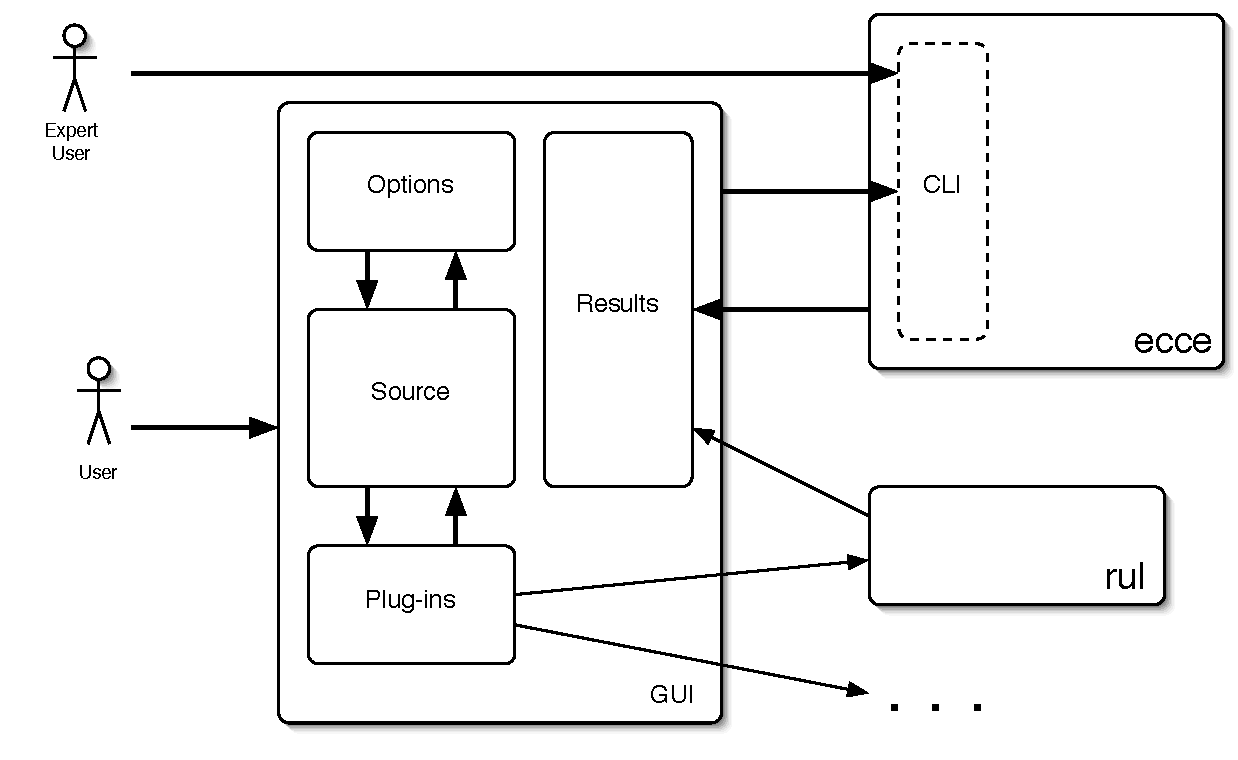
\includegraphics[width=.45\textwidth]{web_ecce}
  \caption{Overall Architecture}\label{fig:php_arch}
\end{figure} 

All of the above actions, as well as the plug-ins, produce an output which is placed underneath the GUI's input \verb!textarea!, with the exception of {\em slicing} that requires some post-processing. Rather than the usual dumping of output code to screen, slicing follows an alternative procedure where the unused clauses of the original code are greyed out. In this way, variable names and comments from the source code are kept, which provides
 better visual feedback to the user.

Another feature available in the GUI, is a visualisation window that can be used to obtain more information about the specialisation process.
By clicking a button, the user can open a new window that displays a graph corresponding to the specialisation tree (see Fig.~\ref{fig:svg}). This graph is 
 first generated by {\sc ecce} in {\tt .dot} format and then  translated to {\tt .svg} format for web displaying.

\begin{figure}[!ht]
  \centering
  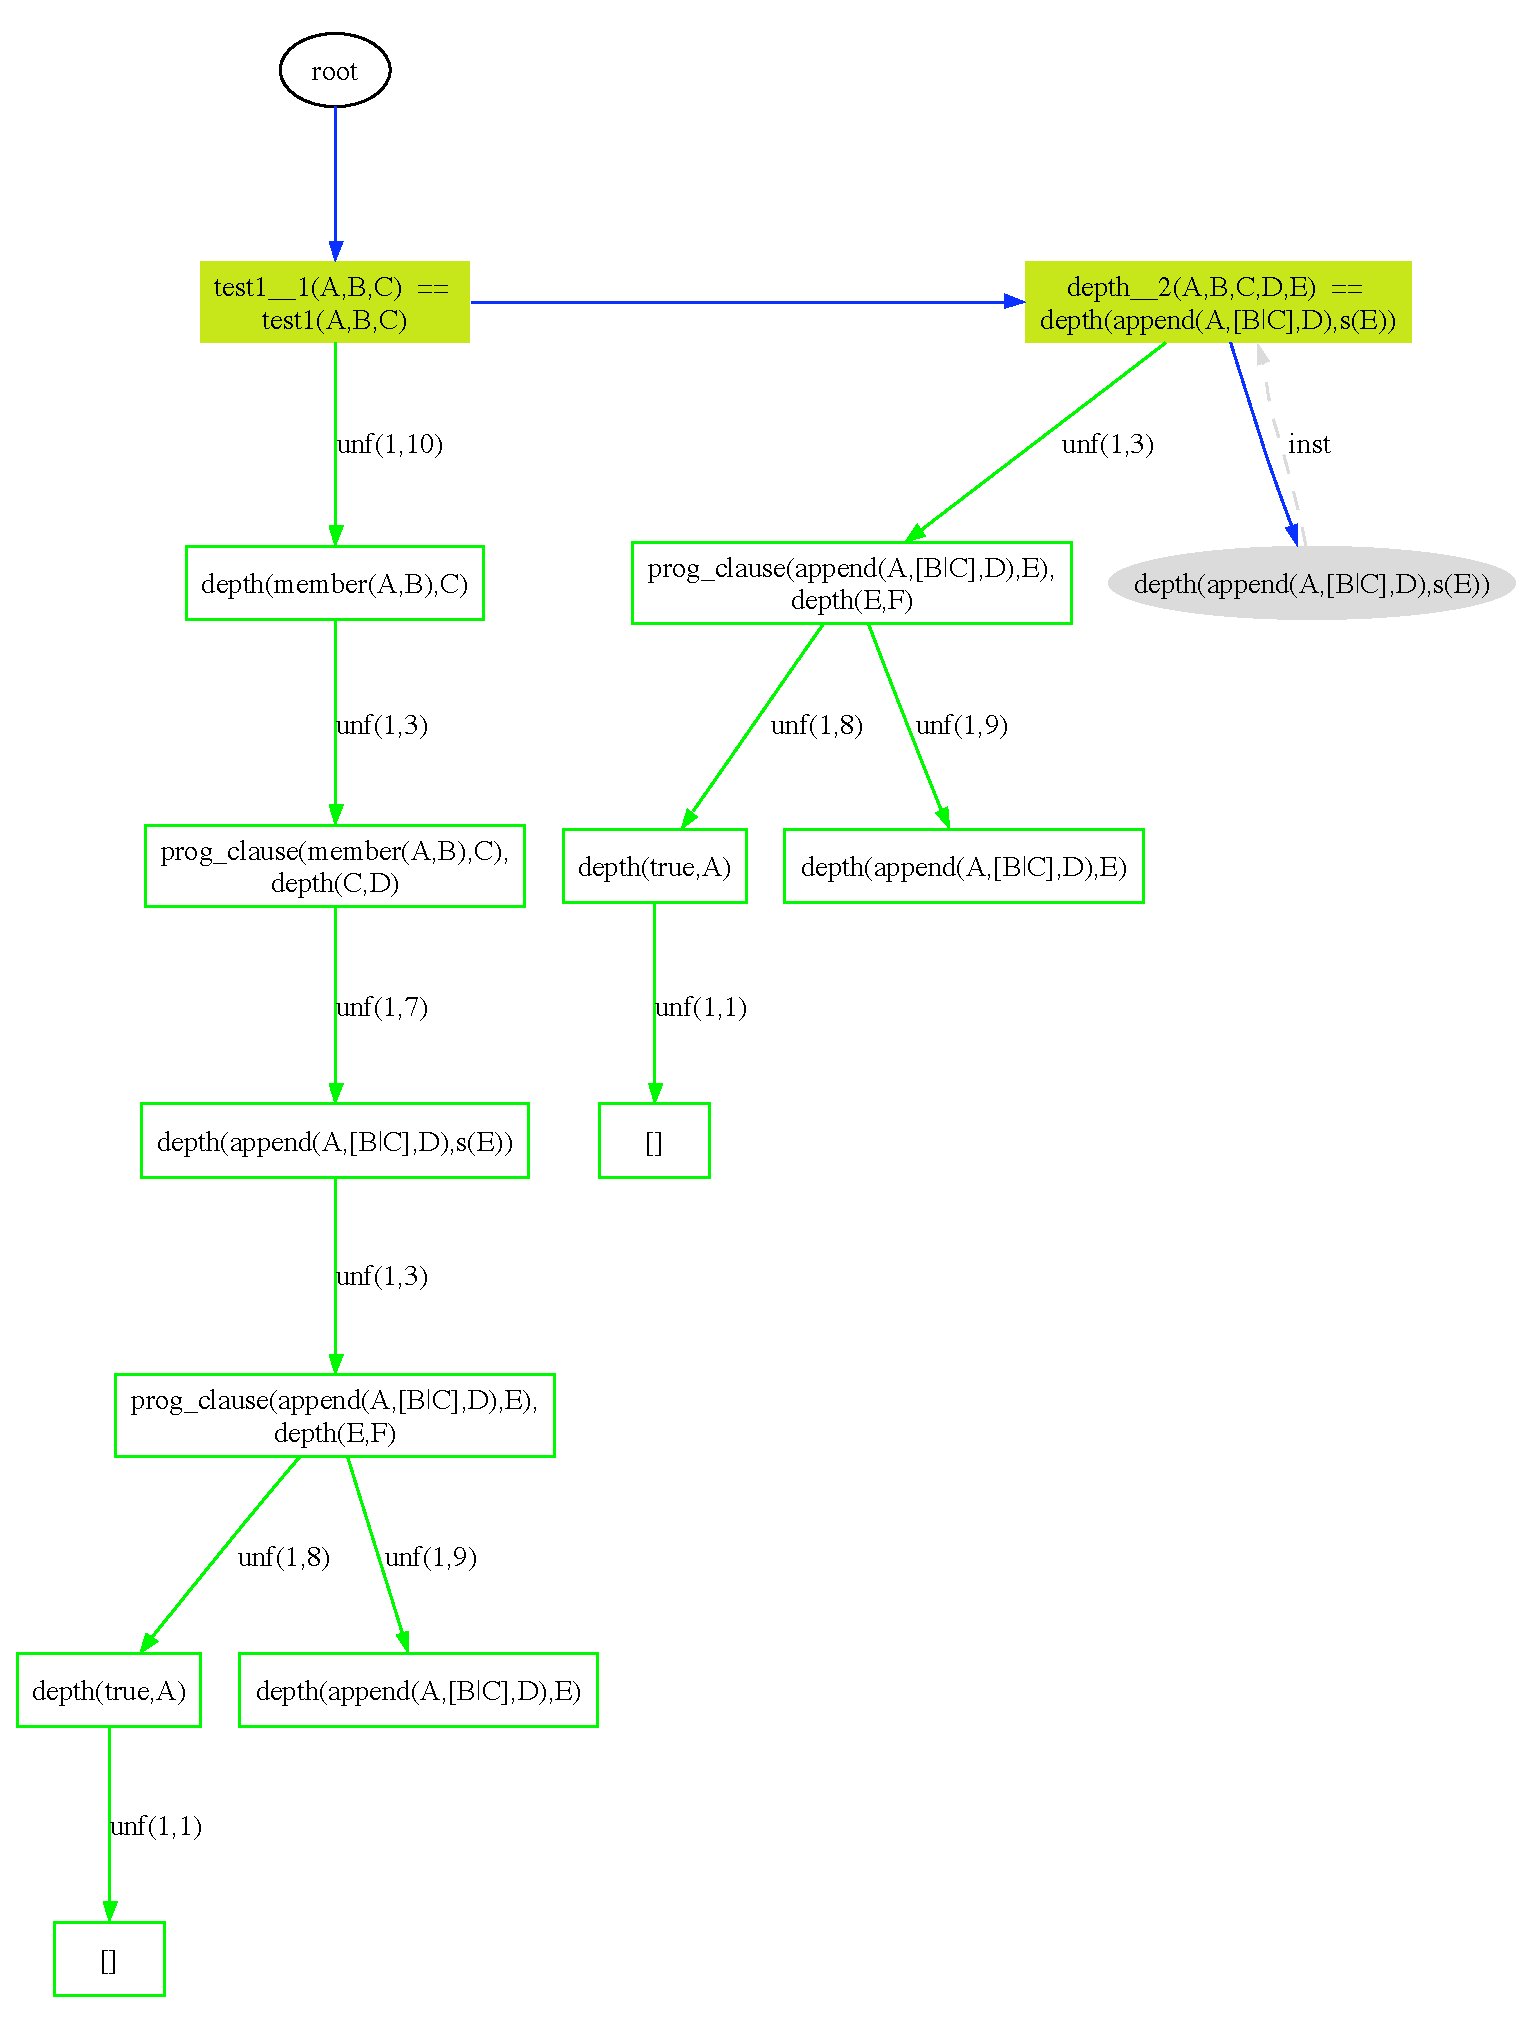
\includegraphics[width=.5\textwidth]{Spectree}
  \caption{Specialisation Tree}\label{fig:svg}
\end{figure} 

As far as security is concerned,
 {\sc ecce} contains a whitelist of built-in predicates with conditions on when it is allowed to evaluate them.
This whitelist is used to ensure that malicious Prolog code submitted to the web interface cannot corrupt the web server.
In addition, a timeout is used to put an upper limit on the resource usage of the web server (for complex specialisation
 tasks users should download and install a local copy of {\sc ecce}.)


\section{Conclusion}

In conclusion, the {\sc ecce}  system provides advanced specialisation for pure Prolog programs.
Being an online specialiser, its usage is simple and accessible to non-expert users. 
The development of the web interface provides an even simpler way of using the system,
 requiring no local installation and providing easy access to various options of the system.
The {\sc ecce} system has been applied to numerous case studies, and has found applications outside
 of its original goal area of specialising programs, e.g., especially for the analysis and verification of systems
  expressed as Prolog rules.
 

\bibliographystyle{abbrv}
\bibliography{michael}

\appendix

\section{Tool Web Site}

\noindent
The main web site for our tool is:\\
{\small\tt http://stups.cs.uni-duesseldorf.de/\~{}pe/ecce}

%\newpage

\section{Presentation Outline}

\begin{enumerate}
\item Introduction
  \begin{itemize}
  \item Partial Evaluation for Prolog
 \item Online Partial Evaluation
        \begin{itemize}
    \item Local vs Global Control
    \item Local and Global Termination
    \item Correctness criteria and results
   \end{itemize}
    \item Conjunctive Partial Deduction
  \end{itemize}
 
 \item Description of the {\sc ecce} Algorithm for Online Partial Evaluation
  \begin{itemize}
    \item Local Control
       \begin{itemize}
    \item Determinacy
    \item Lookahead
    \item Homeomorphic embedding
     \end{itemize}
    \item Global Control
           \begin{itemize}
    \item Characteristic Trees
    \item Homeomorphic embedding
    \end{itemize}
  \end{itemize}
  
  
 \item A simple Example, Complete walk-through
  \begin{itemize}
    \item Source program vanilla meta-interpreter
    \item Specialised program for various static inputs, showing, e.g., 
     that multiple layers of interpretation get removed.
    \item Runtime Results
    \item Different Interfaces:
     \begin{itemize}
    \item The old text menu interface
    \item The Command-Line Interface
    \item The Web Interface
    \end{itemize}
  \end{itemize}
  
  \item Implementation of {\sc ecce} in Ciao
    \begin{itemize}
    \item Modularity
    \item Keeping compatability with both SICStus and Ciao
    \item Development of the command-line interface
   \end{itemize}
  
  \item The Architecture of the Web Interface
    \begin{itemize}
    \item Overall architecture
    \item PHP Implementation
    \item Security aspects
  \end{itemize}
      
 \item Various examples
     \begin{itemize}
    \item Deforestation example
    \item Tupling example
    \item Higher-order example (e.g., map, reduce)
  \end{itemize}
  
   \item Slicing:
     \begin{itemize}
    \item Describe the basic principles:
       \begin{itemize}
    \item What is slicing
    \item How is {\sc ecce} adapted to perform the slicing
    \end{itemize}
    \item Walk through a simple and more complicated example
    \begin{itemize}
    \item 
     highlight precision of approach (individual clauses/facts
     are sliced out)
     \item show visual feedback of web interface
    \end{itemize}
    \end{itemize}
  
 \item Using {\sc ecce} for verification/model checking
  \begin{itemize}
    \item Basic principle: system has to be expressed as
     Prolog rules
      \begin{itemize}
        \item Show Petri net encoding
        \item Show CTL encoding
        \item Possibly show CSP or other more complicated formalism
       \end{itemize}
    \item  Show that {\sc ecce}'s algorithm can be used
     to perform a precise flow/reachability analysis
    \item Show how the most specific version abstract interpretation
     phase can be used to extract the analysis result
  \end{itemize}
    
    
 \item Summary of other Applications
    \begin{itemize}
    \item Summary of experimental results, comparison against 
     mixtus, sp and paddy.
    \item Fluent Calculus
    \item Termination analysis, usage of {\sc ecce} by Codish and Serbrenik
   \end{itemize}
  
  
\end{enumerate}

\newpage
\section{A Screenshot}
~\\
%\begin{figure*}[!ht]
\centering
\begin{minipage}[t]{\textwidth}
  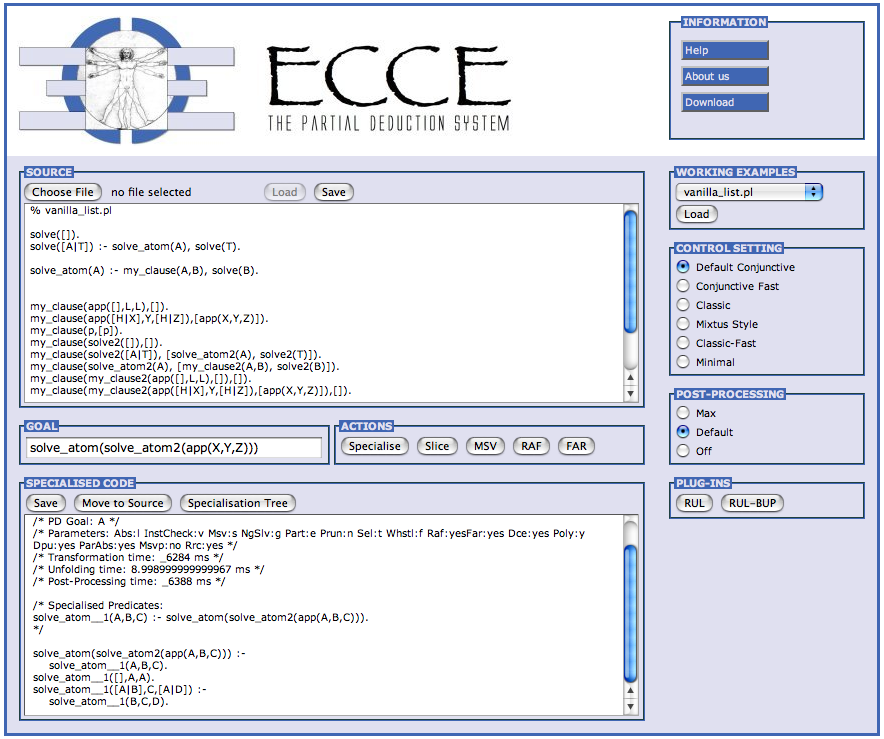
\includegraphics[width=\textwidth]{Screenshot_ecce}
\end{minipage}
%\end{figure*}

%\newpage
%\section{A Specialisation Tree}

%~\\
%%\begin{figure*}[!ht]
%\centering
%\begin{minipage}[t]{.9\textwidth}
%  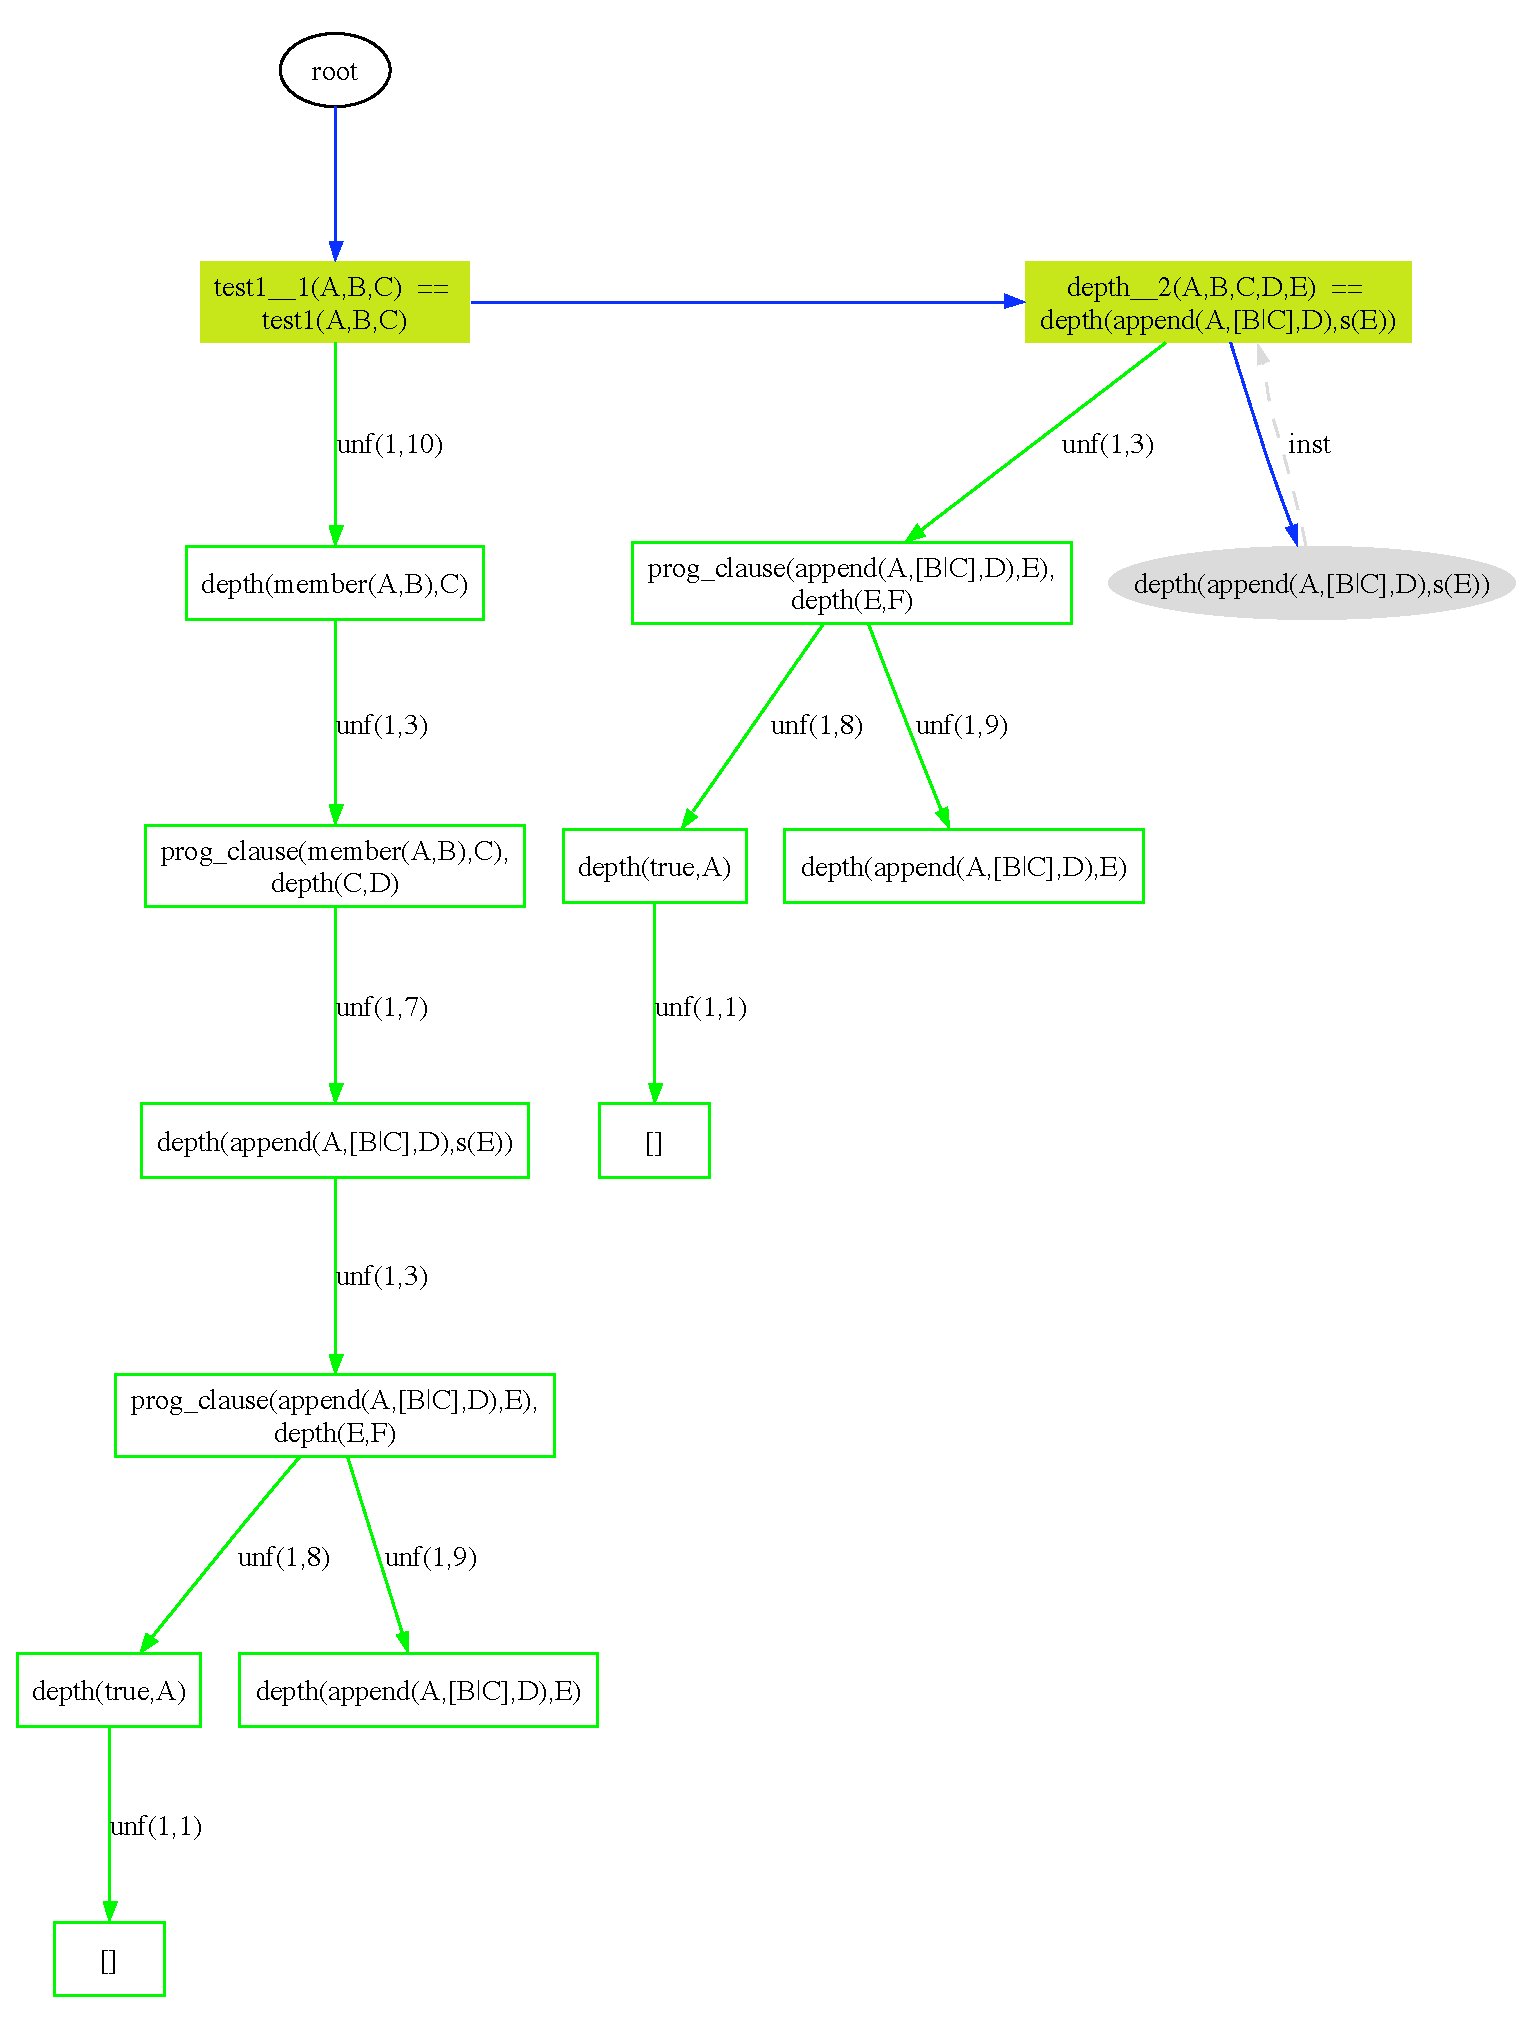
\includegraphics[width=.9\textwidth]{Spectree}
%\end{minipage}
%%\end{figure*}


 \end{document}
 \end
 
